\section{1. Reader Orientation}\label{reader-orientation}

This section explains how to use the index, what kind of repo surface it
covers, and how the pinned-commit source policy affects citations.

\subsection{1.1 Reading lanes and audience
fit}\label{reading-lanes-and-audience-fit}

This subsection gives four practical reading lanes so new readers do not
have to infer a path from folder names alone.

Start here: first-time operators should begin with
\href{https://github.com/chris-page-gov/mcp-geo/blob/fe862910da246ca77f374cfbe484985f5df4d316/README.md\#L1-L240}{README.md},
technical reviewers should jump to
\href{https://github.com/chris-page-gov/mcp-geo/blob/fe862910da246ca77f374cfbe484985f5df4d316/server/main.py\#L1-L216}{server/main.py}
and
\href{https://github.com/chris-page-gov/mcp-geo/blob/fe862910da246ca77f374cfbe484985f5df4d316/server/mcp/tools.py\#L1-L260}{server/mcp/tools.py},
evidence-oriented readers should open
\href{https://github.com/chris-page-gov/mcp-geo/blob/fe862910da246ca77f374cfbe484985f5df4d316/docs/reports/README.md\#L1-L71}{docs/reports/README.md},
and publication editors should move straight to
\href{https://github.com/chris-page-gov/mcp-geo/blob/fe862910da246ca77f374cfbe484985f5df4d316/docs/public_sector_ai_community/README.md\#L1-L60}{docs/public\_sector\_ai\_community/README.md},
\href{https://github.com/chris-page-gov/mcp-geo/blob/fe862910da246ca77f374cfbe484985f5df4d316/docs/spec_package/README.md\#L1-L45}{docs/spec\_package/README.md},
and
\href{https://github.com/chris-page-gov/mcp-geo/tree/fe862910da246ca77f374cfbe484985f5df4d316/docs/mcp_geo_prism_bundle}{docs/mcp\_geo\_prism\_bundle/}.

Where to go:
\href{https://github.com/chris-page-gov/mcp-geo/tree/fe862910da246ca77f374cfbe484985f5df4d316/docs/public_sector_ai_community}{community
documentation set},
\href{https://github.com/chris-page-gov/mcp-geo/tree/fe862910da246ca77f374cfbe484985f5df4d316/docs/spec_package}{specification
package},
\href{https://github.com/chris-page-gov/mcp-geo/blob/fe862910da246ca77f374cfbe484985f5df4d316/docs/reports/README.md}{reports
index}, and
\href{https://github.com/chris-page-gov/mcp-geo/blob/fe862910da246ca77f374cfbe484985f5df4d316/docs/tool_catalog.md\#L1-L61}{tool
catalog}.

\begin{figure}
\centering
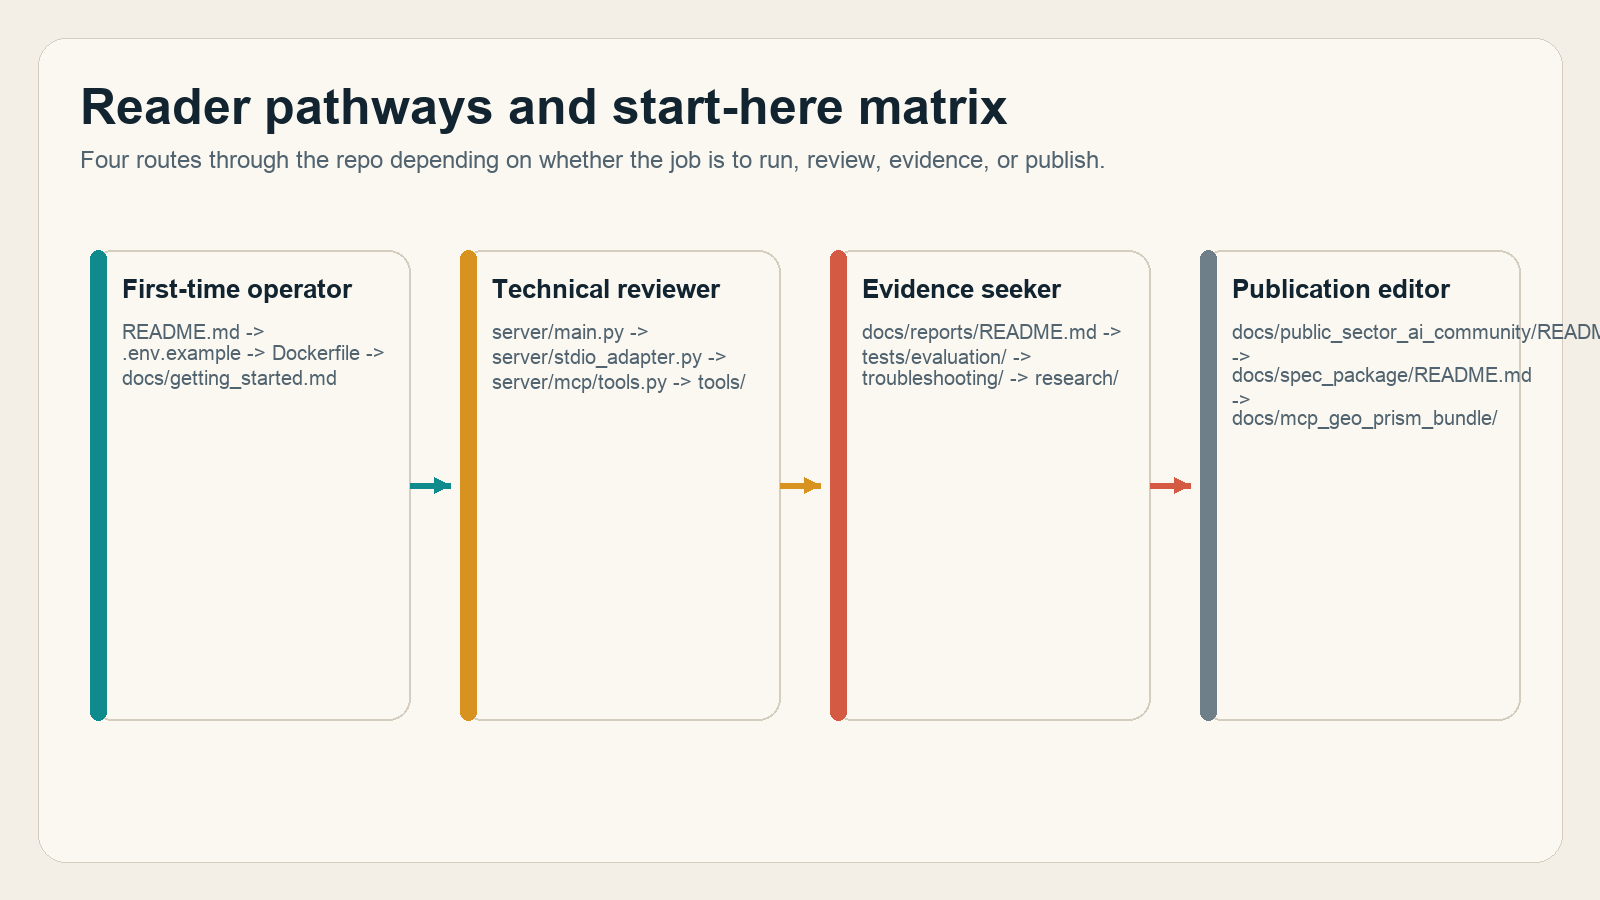
\includegraphics[width=0.96\linewidth,height=\textheight,keepaspectratio,alt={Figure F02. Reader pathways and start-here matrix}]{figures/f02_reader_pathways.png}
\caption{Figure F02. Reader pathways and start-here matrix}
\end{figure}

Figure F02 shows the fastest route for four reader types: operator,
reviewer, evidence seeker, and publication editor.

\subsection{1.2 Citation baseline and source
policy}\label{citation-baseline-and-source-policy}

This subsection makes the evidence rules explicit so readers can tell
which materials are public repo evidence and which are merely contextual
inputs.

The stable source surface is the pinned GitHub repo at
\href{https://github.com/chris-page-gov/mcp-geo/tree/fe862910da246ca77f374cfbe484985f5df4d316}{commit
\texttt{fe862910da246ca77f374cfbe484985f5df4d316}}, and the key baseline
inputs inside that commit are the
\href{https://github.com/chris-page-gov/mcp-geo/blob/fe862910da246ca77f374cfbe484985f5df4d316/docs/slides/20260225\%20-\%20From_Apps_to_Answers.pdf}{slide
deck}, the
\href{https://github.com/chris-page-gov/mcp-geo/blob/fe862910da246ca77f374cfbe484985f5df4d316/docs/reports/mcp_geo_ai_community_event_record.docx}{event
record DOCX}, and the
\href{https://github.com/chris-page-gov/mcp-geo/blob/fe862910da246ca77f374cfbe484985f5df4d316/docs/mcp_geo_prism_bundle/main.md\#L1-L292}{rough
initial Prism bundle}. The external transcript at
\texttt{/Users/crpage/Downloads/20260225-AI-Community-MCP-Talk.txt} is
deliberately excluded from formal citation because it is outside the
pinned public corpus.

Where to go:
\href{https://github.com/chris-page-gov/mcp-geo/tree/fe862910da246ca77f374cfbe484985f5df4d316}{pinned
repo root},
\href{https://github.com/chris-page-gov/mcp-geo/blob/fe862910da246ca77f374cfbe484985f5df4d316/docs/mcp_geo_prism_bundle/main.md\#L122-L292}{rough
bundle baseline}, and
\href{https://github.com/chris-page-gov/mcp-geo/blob/fe862910da246ca77f374cfbe484985f5df4d316/docs/reports/mcp_geo_ai_community_event_record.docx}{event-record
source document}.

\subsection{1.3 What this index does
differently}\label{what-this-index-does-differently}

This subsection states the editorial shift from a short appendix to a
full navigational system with a stronger visual and validation layer.

The earlier Appendix A in the rough Prism bundle already recognized the
repo's main reading zones, but it stopped too early in the deeper
report, testing, and release surfaces and did not record the design
prompts behind its visuals. This replacement keeps the curated approach,
but it accounts for every top-level tracked area at the pinned commit,
adds stable source rules, interleaves a larger visual layer, and records
one regeneration prompt per infographic.

Where to go:
\href{https://github.com/chris-page-gov/mcp-geo/blob/fe862910da246ca77f374cfbe484985f5df4d316/docs/mcp_geo_prism_bundle/main.md\#L122-L292}{previous
Appendix A start},
\href{https://github.com/chris-page-gov/mcp-geo/blob/fe862910da246ca77f374cfbe484985f5df4d316/docs/reports/README.md\#L1-L71}{report
library index}, and
\href{https://github.com/chris-page-gov/mcp-geo/blob/fe862910da246ca77f374cfbe484985f5df4d316/docs/public_sector_ai_community/README.md\#L1-L60}{community
documentation set overview}.
